\documentclass[twocolumn]{article}

\usepackage{graphicx}
\usepackage{amsmath}
\usepackage{amsthm}
\usepackage{amssymb}
\usepackage{url}
\usepackage{multirow}
\usepackage{times}
\usepackage{fullpage}
\usepackage{algorithm}
\usepackage{algpseudocode}

\urlstyle{rm}

\newcommand{\comment}[1]{}

\algrenewcommand{\algorithmicrequire}{\textbf{Input:}}
\algrenewcommand{\algorithmicensure}{\textbf{Output:}}
\algrenewcommand{\algorithmicforall}{\textbf{for each}}

\title{CS615: Group 4 \\ Representative Skylines with Noisy Comparisons}
\author{
\begin{tabular}{cc}
	Pranshu Gupta & Rahul Tudu \\
	13493 & 13538 \\
	\url{pranshug@iitk.ac.in} & \url{trahul@iitk.ac.in} \\
	Dept. of CSE & Dept. of CSE \\
	\multicolumn{2}{c}{Indian Institute of Technology, Kanpur}
\end{tabular}
}
\date{Final report \\	% replace by ``initial'' or ``final'' as appropriate
21st November, 2016}	% replace by actual date of submission or \today

\begin{document}

\maketitle

\begin{abstract}
	%
	Most systems focus on efficiently finding out skylines and the user is presented with the entire set. Now, if the skyline set it large, it becomes the job of the user to manually inspect the points and pick out the most informative ones. These are the representative skyline points. Our system assumes a computation model where the data items can only be compared through noisy comparisons. In this model, for each comparison we have a probability with which the first item will dominate second. A generic system won't work with such model. We intend to implement a system which finds out representative skylines on data with noisy comparison model
	%
\end{abstract}

\section{Problem Statement}

The objective of the implemented system is to find out Representative Skylines on data with Noisy Comparisons.
\begin{center}
    \begin{tabular}{ | l | p{6cm} |}
    \hline
    Input & Description \\ \hline
    $D$ & Number of Dimensions \\ \hline
    $D_i$ & Number of possible values in dimension $i$ \\ \hline
    $M_i$ & Dominance probability matrix for values in dimension $i$. M_i[p,q] = Prob(p \succ q) \\ \hline
    $e$ & Error tolerance for a single comparison \\ \hline
    $N$ & Number of samples in the data \\ \hline
    $Data$ & Samples for which the skyline has to be computed \\ \hline
    \end{tabular}
\end{center}
\begin{center}
    \begin{tabular}{ | l | p{6cm} |}
    \hline
    Output & Description \\ \hline
    $R$ & Skyline Set in Representative Order \\ \hline
    \end{tabular}
\end{center}
\begin{center}
    \begin{tabular}{ | l | p{6cm} |}
    \hline
    Notation & Description \\ \hline
    $S$ & Skyline Set \\ \hline
    $W_i$ & A sorted instance of the values in dimension $i$ as per $M_i$ \\ \hline
    $LD$ & Data labeled according to $W$ \\ \hline
    $DS$ & Dominance sets for the skyline points \\ \hline
    $J$ & Jaccard distance matrix for the skyline set $S$ \\ \hline
    \end{tabular}
\end{center}

\subsection{Related Material}
The work by Groz and Milo \cite{skyline} talks about finding skylines for data with noisy comparisons based on the model described in the paper by Feiget et al. \cite{noisy}. A procedure to find out representative skylines on absolute data is described in the paper by Valkanas et al. \cite{represent}. We combine these two works \cite{skyline}, \cite{represent} to find out representative skylines for data with noisy comparisons.

\section{Approach}
Finding representative skylines with noisy comparisons involves the sorting the possible values in the dimension according to the noisy comparison model. Our system does merge sort with a custom comparison operator. This operator takes two points $p$ and $q$ and the uses the dominance probability matrix for the corresponding dimension, and does repetitive comparisons with each comparison giving the result according to the value in $M_i$[p,q]. The result given by the operator is decided by the majority vote of the repetitive comparisons. So, if majority says $p \succ q$ then the operator says $p \succ q$. \cite{noisy}

After the sorting of the possible values in each dimension is done, the attributes of the data points are labeled accordingly. Say, if a value $p$ in dimension $d$ comes at position $i$ in the sorted order then all the instances of $p$ in dimension $d$ the data points will be labeled as $i$.

Now, the attributes so labeled are assumed to represent the numeric values of the data points and thus, we can utilize any skyline finding algorithm on the labeled data. Our system uses SFS algorithm for this purpose. \cite{skyline}

After we have found the skyline set, we find the dominance sets of each skyline point. These dominance sets are used to find out the pairwise Jaccard distances of the skyline points. Jaccard distance is defined as the ratio of sizes of the intersection to the union of the dominance sets of the concerned points. 

Finally, to find the representative order of the skylines we follow the Jaccard Distance based diversification algorithm. The skyline point with largest domination is chosen as the initial point in cluster $A$. Then in every iteration, we choose the next skyline point $q$ such that minimum Jaccard distance of $q$ to any $p$ in the cluster $A$ is maximized. We already have computed jaccard distances so we don't use min-hashing for estimation. Ties are broken using the domination score.
\cite{represent} \\

The main algorithm followed by our system is RSNC (see Algorithm 1)

\begin{algorithm}[t]
	\caption{RSNC}
	\label{alg:indexing}
	\begin{algorithmic}[1]
		\Require $D$, $D_i$, $M_i$, $e$, $N$, $Data$
		\Ensure Result set $R$
		\State Foeach $i$: $W_i \gets$ $D_i$.Sort($M_i$, e)
		\State $LD \gets$ $Data$.Label($W$)
		\State $S \gets$ $LD$.SFS()
		\State Foreach $p$ in $S, DS[p] \gets p$.DominanceSet($LD$)
		\State Foreach (p,q): J[p,q] $\gets $JaccardDist(p,q)
		\State Find the Respresentative order of $S$ using the jaccard distance based diversification algorithm and store the result in $R$
		\State Return $R$
	\end{algorithmic}
\end{algorithm}

\section{Results}
We have tested our implementation for different use cases. For example, how does the size of skyline set change when we increase the number of samples in the data. How much time does the system take to compute the result with varying sample sizes. Please see Figure \ref{fig:size} and Figure \ref{fig:time} for the results. Note that both of these plots were obtained on varying the sample size while keeping the comparison model constant (with 5 independent dimensions, each having 20 possible values) and error tolerance ($e$) equal to 0.1 with 100 runs for each sample size (for sizes above 10000, 10 runs were done).
 
\begin{figure}[t]
	\centering
	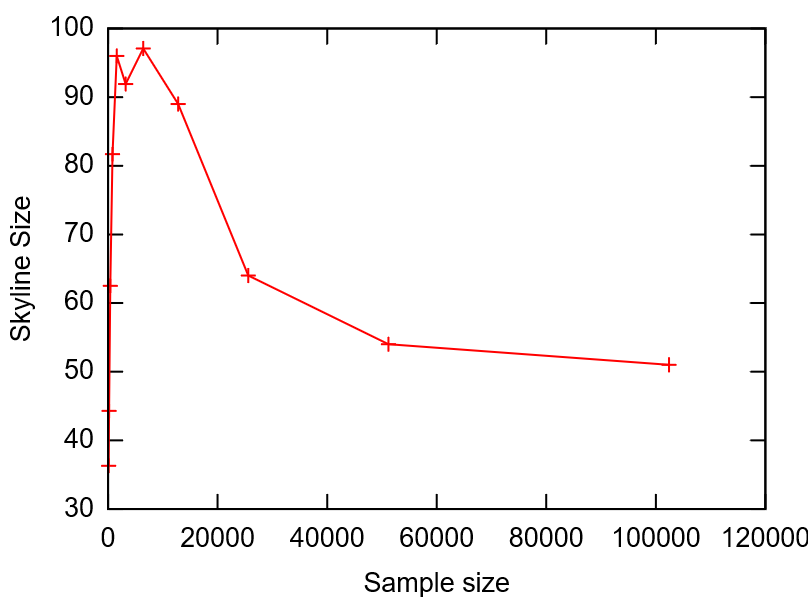
\includegraphics[width=0.98\columnwidth]{skysize.png}
	\caption{Average Number of Skylines vs Sample Size}
	\label{fig:size}
\end{figure}

We can see in Figure \ref{fig:size} that the number of skylines first  increases as we increase the number of samples but for very large number of samples it starts decreasing and then becomes stable. 

This is because the domain of possible values in each dimension is finite and as we go on increasing the number of samples, the possibility of a dominating point being there in the data first increases and for very large set most of the dominating point are there so the number of skylines flattens out. Initially, the number of skylines does increase when the data size is smaller as in that case most of the points are of similar calibre and hence, incomparable.

So, now we increase the number of possible values in each dimension while keeping the sample size constant. The following table shows that number of skylines increases with increase in the domain size of the dimensions. This in turn supports our claim about the no. of skylines w.r.t the sample size.

\begin{center}
    \begin{tabular}{ | l | l | l |}
    \hline
    Samples & Domain Size per Dim. & No. of Skylines \\ \hline
    25600 & 10 & 1 \\ \hline
    25600 & 20 & 63 \\ \hline
    25600 & 30 & 110 \\ \hline  
    25600 & 40 & 161 \\ \hline
    25600 & 50 & 235 \\ \hline
    25600 & 60 & 236 \\ \hline
    25600 & 100 & 247 \\ \hline
    \end{tabular}
\end{center}

We also analyzed how the results changed on varying the number of dimensions while keeping the number of samples constant. The following table shows the results when the number of samples ($N$) was 12800, $e$ = 0 and domain size for each dimension $D_i$ = 20. The number of skylines increases with increasing number of dimensions. This is what we call the curse of dimensionality.

\begin{center}
    \begin{tabular}{ | l | l | l | l |}
    \hline
    #Samples & #Dimensions & #Skylines & Time(s) \\ \hline
    12800 & 5 & 59 & 30.86\\ \hline
    12800 & 6 & 259 & 45.96\\ \hline
    12800 & 7 & 823 & 190.67\\ \hline  
    12800 & 8 & 1504 & 1212.11\\ \hline
    12800 & 9 &  2776 & 12323.2\\ \hline
    \end{tabular}
\end{center}


The total time taken to compute the result increases with the number of samples as expected.

\begin{figure}[t]
	\centering
	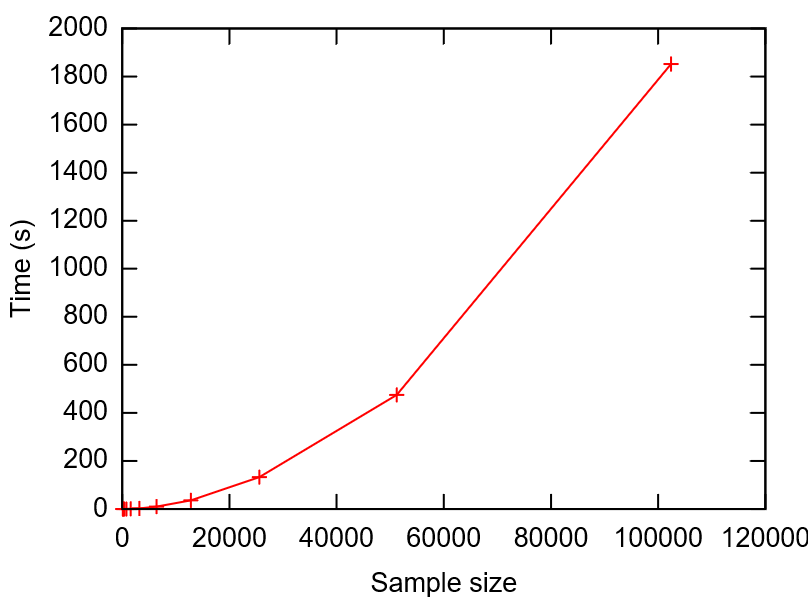
\includegraphics[width=0.98\columnwidth]{time.png}
	\caption{Time taken vs Sample Size}
	\label{fig:time}
\end{figure}

There is one more important parameter in our implementation, the error tolerance of the comparison model ($e$). We also tested how the results differ on changing the value of $e$. 

On increasing the tolerance of the comparison operator the skyline many other points which were not in the true skyline set ($e$ = 0) also creep into the result set. Also, the representative ordering does not seem to be preserved. As we can see in Figure \ref{fig:0.1} which plots the scores of each skyline point in with $e$ = 0 and $e$ = 0.1.

Score of a point is defined as the sum of the reciprocal of representative ranks of the point in multiple runs of program. So, better ranks will lead to higher score. Rank is the index of the skyline point in the representative order. 

We can see that the score has been distributed across points with $e$ = 0.1. One of the reason can be that we are applying opposite sided tolerance in each comparison. That is, if dominance probability is greater than 0.5 then we subtract e from it while doing the comparison, otherwise we add e. So, we are making domination more difficult. That is why other points are also becoming skylines.

However, if we keep $e$ = 0 the skyline set remains constant as well as the representative order is preserved in all the runs. 

\begin{figure}[t]
	\centering
	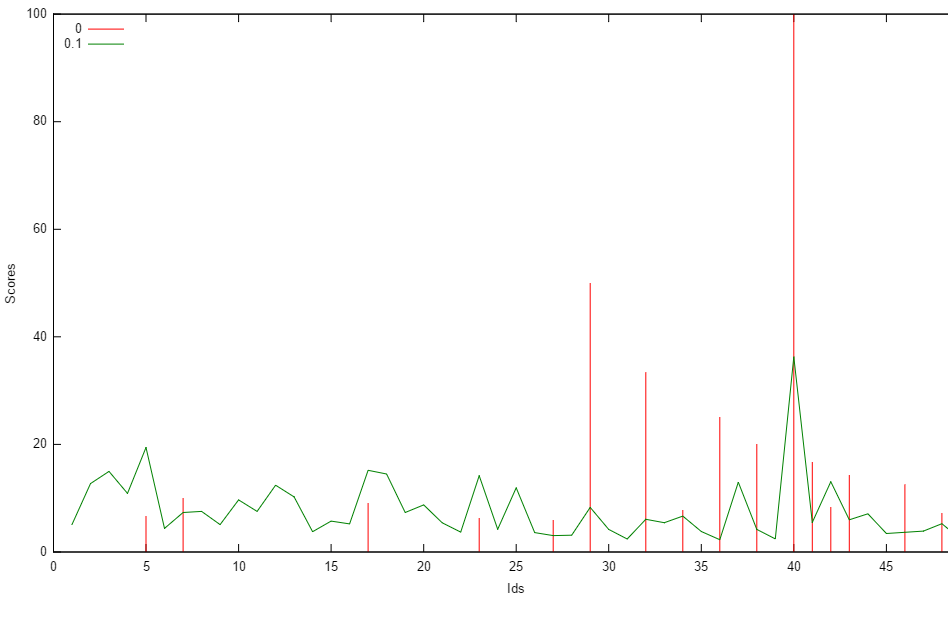
\includegraphics[width=0.98\columnwidth]{1.png}
	\caption{Score of Each ID}
	\label{fig:0.1}
\end{figure}

\comment{

\begin{table}[t]
	\centering
	\begin{tabular}{|c||cc|}
		\hline
		Header 1 & Desc 1 & Desc 2 \\
		\hline
		\hline
		Row 1 & Data 1-1 & Data 1-2 \\
		Row 2 & Data 2-1 & Data 2-2 \\
		\hline
	\end{tabular}
	\caption{Table of results.}
	\label{tab:results}
\end{table}

And refer as Table \ref{tab:results}.

}

\section{Conclusions}

We have successfully implemented and analyzed a system that can give representative skylines on data with noisy comparisons. Suggested future improvements and possible extensions of this work are as follows: 
\begin{itemize}
    \item Optimize the representative order of skylines finding part. The skyline diversification algorithm. Can use the jaccard distance estimation technique.
    \item Enable the program for distributed data-sets
    \item As of now, all the dimensions are assumed to have noisy comparison model. We can add the ability to allow some of the dimensions to have absolute comparisons.
    \item Add ability to read all kinds of input attributes strings, numbers etc. for noisy comparison model.
    \item Add the ability to take the comparison model as a function that can be used to compute the dominance probability (if applicable) and thus avoid storing the dominance probability matrices for each dimension. This will considerably reduce the memory usage. This will also enable us to take inputs which have dimensions with infinite sized domain.
    \item Implement other methods to find representative skylines and enable the user to choose one of them at run-time
    
\end{itemize}

\section{Appendix}
\begin{center}
    \begin{tabular}{ | l | l | l |}
    \hline
    Sample & Avg. No. of Skylines & Time Taken (sec) \\ \hline
    100 & 36.3 & 0.0775685 \\ \hline
    200 & 44.3 & 0.092131 \\ \hline
    400 & 62.5 & 0.133191 \\ \hline
    800 & 81.7 & 0.296066 \\ \hline
    1600 & 96 & 0.891572 \\ \hline
    3200 & 91.9 & 2.89024 \\ \hline
    6400 & 97.1 & 10.165 \\ \hline
    12800 & 89 & 35.932 \\ \hline
    25600 & 64 & 132.972 \\ \hline
    51200 & 54 & 474.988 \\ \hline
    102400 & 51 & 1852.29 \\ \hline
    \end{tabular}
\end{center}

\begin{figure}[H]
	\centering
	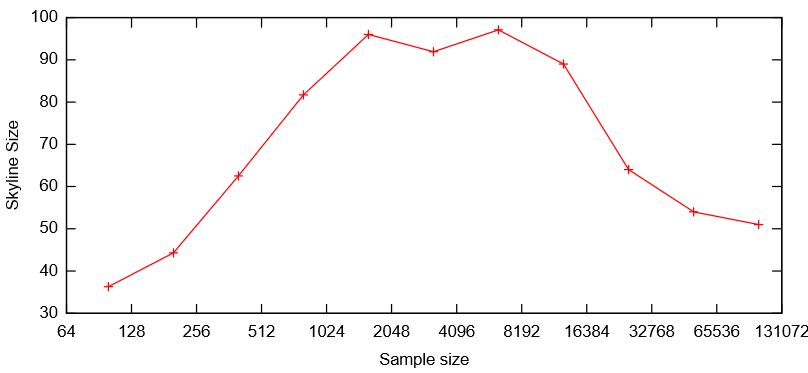
\includegraphics[width=0.98\columnwidth]{sizelog.png}
	\caption{Avg. no. of Skylines vs Sample Size (log scale)}
	\label{fig:sizelog}
\end{figure}

\section{Implementation Details}
We have implemented the entire system in C++11. We have strictly followed the Object Oriented Model of programming. The source code is publicly available on Github under GNU GPL v3.0. You can find the repository at \href{https://github.com/Pranshu258/RSNC}

\section{Usage}
\begin{itemize}
    \item Prepare the Input files
    \begin{itemize}
        \item input/dims : write the number of dimensions in the first line followed by D lines such that i'th next line has the domain size of i'th dimension
        \item input/samples : write the number of samples in the data
        \item input/tolerance : the error tolerance of comparison operator. Choose 0 for best results.
        \item input/data : D lines, line i has the i'th dimension attribute value for all the items in the data sepearted by spaces
        \item input/model : D matrices, matrix i defining the comparison model for i'th dimension. matrix[i][p,q] will contain the probability of p dominating q in dimension i.
    \end{itemize}
    \item Run the program
    \begin{itemize}
        \item If you already have created all the input files then issue the following command \\
        \$ bin/main f f
        \item If you have only created the input files for dims, samples and tolerance and want the program to generate the data and model files for you, issue the following command. \\
        \$ bin/main t t
        \item If you have created the input files for dims, samples tolerance and model and want the program to generate the data file for you, issue the following command \\
        \$ bin/main f t
        \item If you have created the input files for dims, samples tolerance and data and want the program to generate the model file for you, issue the following command \\
        \$ bin/main t f
        \item The program will print the ids of the skyline points in their representative order, along with the number of Skylines and the total time spent in doing the computations.  
    \end{itemize}
    \item Please note that the attribute values in the data file must agree with the number of dimensions and the domain size of each dimension described in the corresponding input files
\end{itemize}


\section{Division of Labor}
Std 1 - Pranshu Gupta: 50 and Std 2 - Rahul Tudu: 50

\begin{thebibliography}{3}

\bibitem{skyline} 
Benoit Groz and Tova Milo. 
\textit{Skyline Queries with Noisy Comparisons}. 
ACM SIGMOD/PODS, May 2015, Melbourne, Australia.
 
\bibitem{noisy} 
Uriel Feiget, Prabhakar Raghavant, David Peleg and Eli Upfal
\textit{Computing with Noisy Information}. 
Society for Industrial and Applied Mathematics, 1994

\bibitem{represent} 
George Valkanas, Apostolos N. Papadopoulos and Dimitrios Gunopulos
\textit{SkyDiver: A Framework for Skyline Diversification}. 


\end{thebibliography}


\end{document}

